%narms.tex, an example driver file for Balkema documents.

%use the following for A4 paper:
\documentclass[12pt,a4paper,twocolumn,fleqn]{narms}

% packages needed
\usepackage{subfigure}
\usepackage{epsfig}
\usepackage{timesmt}
\usepackage{amsmath,setspace}

% add here more packages based on the document format


% setting math equation indent from left 0pts

\mathindent=0pt%

% use this for chicaco style reference
% Author references
% IMPORTANT: Author wants to format references in chicaco style Author must use BiBTex
% IMPORTANT: Author wants to format numbered references remove chicaco style file and \bibliographystyle{chicaco}

\usepackage{chicaco}


%%%%%%%%%%%%%%%%%%%%%%%%%%%%%%%%%%%%%%%%%%%%%%%%%%%%%%%%%%%%%%%%%%
\newcommand{\noin}{\noindent}
\newcommand{\bc}{\begin{center}}
\newcommand{\ec}{\end{center}}
\newcommand{\vc}[1]{\vspace*{#1cm}}
\newcommand{\hc}[1]{\hspace*{#1cm}}
\newcommand{\M}{\mathcal{M}}
\newcommand{\bld}[1]{\boldsymbol{#1}}
\newcommand{\ba}{\bld{a}}
\newcommand{\blc}{\bld{c}}
\newcommand{\bth}{\bld{\theta}}
\newcommand{\bPhi}{\bld{\Phi}}
\newcommand{\bphi}{\bld{\phi}}
\newcommand{\bPsi}{\bld{\Psi}}
\newcommand{\bpsi}{\bld{\psi}}
\newcommand{\bXi}{\bld{\Xi}}
\newcommand{\bxi}{\bld{\xi}}
\newcommand{\beq}{\begin{equation}}
\newcommand{\eeq}{\end{equation}}
%%%%%%%%%%%%%%%%%%%%%%%%%%%%%%%%%%%%%%%%%%%%%%%%%%%%%%%%%%%%%%%%%%

%  \cite{key}
%    which produces citations with full author list and year.
%    eg. (Brown 1978; Jarke, Turner, Stohl, et al. 1985)

%  \citeNP{key}
%    which produces citations with full author list and year, but without
%    enclosing parentheses:
%    eg. Brown 1978; Jarke, Turner & Stohl 1985

%  \citeA{key}
%    which produces citations with only the full author list.
%    eg. (Brown; Jarke, Turner & Stohl)

%  \citeANP{key}
%    which produces citations with only the full author list, without
%    parentheses eg. Brown; Jarke, Turner & Stohl

%  \citeN{key}
%    which produces citations with the full author list and year, but
%    can be used as nouns in a sentence; no parentheses appear around
%    the author names, but only around the year.
%      eg. Shneiderman (1978) states that......
%    \citeN should only be used for a single citation.

%  \shortcite{key}
%    which produces citations with abbreviated author list and year.

%  \shortciteNP{key}
%    which produces citations with abbreviated author list and year.

%  \shortciteA{key}
%    which produces only the abbreviated author list.

%  \shortciteANP{key}
%    which produces only the abbreviated author list.

%  \shortciteN{key}
%    which produces the abbreviated author list and year, with only the
%    year in parentheses. Use with only one citation.

%  \citeyear{key}
%    which produces the year information only, within parentheses.

%  \citeyearNP{key}
%    which produces the year information only.


%%%%%%%%%%%%%%%%%%%%%%%%%%%%%%%%%%%%%%%%%%%%%%%%%%%%%%%%%%%%%%%%%%%
%%%  All this stuff is from modifying the article.cls for Balkema
%%%  specifications.

%\title{...}
%\author{...}
%use \aff for author affiliations
% use \authornext for from second author
% empty line space between multiple authors
%\abstract{...}
%\maketitle{}

%%%%%%% Style for TABLES
% insert tabular command inside \tabletext{} this will produce tables in 10pts


\begin{document}
\title{Metamodeling of structural systems with parametric uncertainty subject to stochastic excitation}
\author{{M. Spiridonakos \& E. Chatzi}\\
{\aff{Institute of Structural Engineering, D-BAUG, ETH Zurich,}} \\
{\aff{Wolfgang-Pauli Str. 15, 8093 Zurich, Switzerland}} }

\date{}% No date.

\abstract{


The problem of estimating reduced order metamodels for the accurate representation of computationally costly numerical models is presently addressed. The introduced metamodeling method is based on Nonlinear AutoRegressive models with eXogenous input (NARX), able to describe nonlinear dynamics, which moreover are characterized by random parameters utilized for the description of the uncertainty propagation. These random parameters are expanded onto a suitably defined finite-dimensional Polynomial Chaos (PC) basis and thus the resulting representation is fully described through a small number of deterministic coefficients of projection. The effectiveness of the proposed method is illustrated through its application on the metamodeling of a five-storey shear frame model paradigm. The results demonstrate the efficiency of the proposed methodology for accurate prediction and simulation of the numerical model dynamics.} 


\maketitle

\section{INTRODUCTION}

The assessment of the dynamic behavior of structural systems subjected to extreme loading conditions, such as earthquakes, is of particular importance for the safe operation of civil structures. Nevertheless, for the vast majority of such structures, it is hardly ever possible to perform dynamic response testing on the actual structure or even realistic simulation tests on an appropriately scaled structural model. 

The advancements achieved in the field of Finite Element (FE) modeling methods have played a key role in overcoming this hurdle by enabling the realization of sophisticated simulation experiments emulating structural response \cite{Bathe2009}. However, despite the rapidly growing computational power and the continuous development of increasingly efficient algorithms, the also growing complexity of FE models and the necessity for more detailed descriptions of both structural geometry and mechanical properties renders the use of highly detailed FE models almost prohibitive for complex, large structures \cite{Gholizadeh-Salajegheh2009}. The problem is even more pronounced when taking into account that the structural systems are commonly characterized by parameter uncertainty to what concerns for instance the mechanical properties of the structure. Thus, the analyst is faced with the task of performing a number of simulations in order to obtain an accurate numerical model of an existing structure. Moreover, when the linearity assumption is relaxed in favor of increased modeling accuracy the numerical model must be tested for a number of different excitation scenarios. Thus, for the extensive experimentation required for design optimization or model updating procedures based on time history loading, a simpler representation of the FE model should be considered which should also be able to describe the behavior of the structure for a wide range of excitations. 

In this work, both structural properties and excitation uncertainties are treated by means of a time-series model with random parameters utilized for the description of uncertainty propagation through the numerical model. More specifically, the random responses of a large-scale numerical model are approximated by a suitably defined Polynomial Chaos Nonlinear AutoRegressive with eXogenous input (PC-NARX) metamodel which is able to describe both types of uncertainties by the expansion of its random model parameters onto a finite-dimensional PC basis \cite{Spiridonakos-Chatzi2012,Blatman-Sudret2010}. Thus, the PC-NARX metamodel is described by a small number of deterministic coefficients of projection, which may be estimated through the ordinary least squares method.

The method's effectiveness is demonstrated through the identification of a metamodel for a five-storey building with nonlinear material properties. Toward this end, a limited number of simulation experiments is conducted with the numerical model being subjected to a number of different realizations of synthetic earthquakes. Synthetic earthquakes are produced by filtering a white noise process through a non-stationary impulse response filter and a non-stationary modulating function in order to simulate the time-varying characteristics for both the temporal and spectral content of a real earthquake \cite{Rezaeian-Kiureghian2010}. The non-stationary filter and the modulating functions are described by a small number of uncertain parameters, with sample observations of the latter being estimated through fitting of the model to real recorded earthquake ground motion signals. 




% ===============================================
\section{POLYNOMIAL CHAOS NARX MODELS}
% ===============================================
\label{sec:PCNARX}

Metamodeling refers to the process of identifying a reduced order and computational complexity representation of a large scale numerical model. In the present work, a metamodel is sought for the accurate representation of the dynamics of the numerical model and the accurate simulation of its time history loading response.

Let us consider a structural system represented by a numerical model $\mathcal M$ that is characterized by a number of input parameters related with the properties of the modeled structure (mechanical and/or geometric). It is assumed that $M_1$ of these parameters are subject to uncertainty and that they may be described by independent random variables gathered in a random vector $\bxi_S = [ \xi_{1}, \xi_{2},\ldots ,\xi_{M_1} ]^{\mathsf T}$. Superscript $\mathsf T$ denotes transpose of a vector or a matrix while it is noted that for simplicity of notation no distinction is made between a random variable and its value(s).


Since the dynamic behavior of a nonlinear numerical model is also a function of the input excitation characteristics, it is considered that the set of excitation signals used for the dynamic loading of the numerical model may be described by a small number of random variables $\bxi_X = [ \xi_{M_1+1}, \xi_{M_1+2},\ldots ,\xi_{M_1+M_2} ]^{\mathsf T}$. 

As a result of the uncertainty propagation, the dynamic response of the numerical model to a given input excitation will also be a random variable which in addition depends on time, that is
%%
\beq 
y[t,\bxi] = {\mathcal M}(x[1,\bxi_X],x[2,\bxi_X],\ldots,x[t,\bxi_X],\bxi_S)
\eeq
%%
with $t = 1,2,\ldots, T $ designating normalized by the sampling period discrete time, $x[t,\bxi_X]$ the excitation input signal, $y[t,\bxi]$ the corresponding numerical model response signal, and $\bxi = [ \bxi_S^\mathsf{T} \ ,\ \bxi_X^\mathsf{T} ]^\mathsf{T}$ the $M$-dimensional ($M = M_1 + M_2$) complete vector of input random variables with known joint probability density function (pdf) $f(\bxi)$ . 

In order to approximate the numerical model dynamic response $y[t,\bxi]$ for every realization of $\bxi$ in an efficient way, a novel metamodeling method based on Polynomial Chaos Nonlinear AutoRegressive with eXogenous input (PC-NARX) models is introduced in the present study. The general PC-NARX model, in the linear-in-the-parameters form, is given by the following relationship:
%%
\beq y[t] =  \sum_{i=1}^{n_\theta} \theta_i(\bxi) \cdot g_i({\bld z}[t]) + e[t] \label{eq:PCNARX}\eeq
%%
where $g_i({\bld z}[t])$ are the nonlinear model terms generated from the regression vector ${\bld z}[t] = \bigl[ y[t-1],$ $\ldots, y[t-n_a], $ $x[t],\ldots ,x[t-n_b] \bigr]^\mathsf{T}$ with $n_a, n_b$ designating the maximum output and input time lags, respectively, and $e[t]\! \sim\! \text{NID} (0,\sigma^2_e)$ the model's residual sequence with NID$(\cdot,\cdot)$ denoting Normally Independently Distributed process with the indicated mean and variance. It should be mentioned that the model terms $g_i({\bld z}[t])$ may be constructed from a variety of local or global basis functions including polynomials, splines, neural networks, wavelets and others \cite{Wei-Billings2009}.

The important feature of PC-NARX models, in comparison with the conventional NARX models \cite{Chen-Billings1989}, is that they are characterized by parameters $\theta_i(\bxi)$ which are random variables themselves. The latter are actually represented by a deterministic mapping which describes their relation with the input random variables. More specifically, assuming that the PC-NARX model parameters $\theta_i(\bxi)$ have finite variance, they admit the following polynomial chaos representation \cite{Soize-Ghanem2004}:
%%
\beq 
\theta_i (\bxi) = \sum_{j=1}^{\infty } \theta_{i,j}\cdot \phi_{\bld{d}(j)}(\bxi) \label{eq:PCE}
\eeq
%%
where $\theta_{i,j}$ are unknown deterministic coefficients of projection, ${\bld d}{(j)}$ is the multi-indices of the multivariate polynomial basis, and $\phi_{{\bld d}(j)}$ are multivariate basis functions that are orthonormal with respect to the joint pdf of $\bxi$, that is:
%%
\beq
E[ \phi_{\bld \alpha} (\bxi), \phi_{\bld \beta} (\bxi) ] = \delta_{{\bld \alpha},{\bld \beta}} =\begin{cases} 1 & \mbox{for } \alpha = \beta \\ 0 & \mbox{otherwise} \end{cases}
\eeq
%%
Each probability density function may be associated with a well known family of orthogonal polynomials. For instance, normal distribution is associated with Hermite polynomials while uniform distribution with Legendre. A list of the most common probability density functions along with the corresponding orthogonal polynomials and the relations for their construction may be found in \cite{Soize-Ghanem2004}.

For purposes of practicality, the infinite series of expansion of equation (\ref{eq:PCE}) must be truncated by selecting an appropriate functional subspace consisting of a finite number of terms $p$. In this way, the resulting PC-NARX model is fully parametrized in terms of a finite number of deterministic coefficients of projection $\theta_{i,j}$, while the complete PC-NARX identification problem consists of the subproblems of model parameter estimation and model structure selection, which are discussed in the following sections.

At this point it should be noted that PC-ARIMA models with a-priori known deterministic coefficients of projection have been considered before for the characterization of terrain topology by Wagner and Ferris \cite{Wagner-Ferris2007}. Moreover, linear PC-ARX models have used in the metamodeling context in \cite{Spiridonakos-Chatzi2012}. Similarly linear ARX models with functionally dependent parameters have also been used in a number of studies for the purposes of structural identification and damage detection (for instance see \citeNP{Kopsaftopoulos-Fassois2012} and the references therein). However, in these studies the input parameters are not related with a known probability density function and thus the basis is constructed from an arbitrarily selected family of orthogonal basis functions.


%=========================================================================
\subsection{Parameter estimation}\label{sec:MPE}
%=========================================================================

As already mentioned, the estimation of a PC-NARX metamodel refers to the determination of the coefficients of projection parameter vector $\bth$ 
%%
\beq \bth = [\, \theta_{1,1} , \, \theta_{1,2}, \, \ldots ,\, \theta_{n_\theta,p} \, ]^{\mathsf T} \eeq 
%%
The calculation is based on the availability of time history data for the input excitation and output response of the numerical model. These may be acquired for a series of simulations, conducted for different realizations of the input random vector using the full scale numerical model.


Let us consider a series of $K$ simulations conducted for a corresponding number of input random vector realizations $\bxi_k = [\xi_{k,1}, \xi_{k,2}, \ldots ,\xi_{k,M}]^{\mathsf T}$ (for $k=1,2,\ldots,K$), and the resulting set of set of excitation signals $x_k^T = \{ x_k[1], x_k[2], \ldots, x_k[T] \}$. It is noted that for the purposes of notational simplicity the dependency of the input and output signals on $\bxi_k$ is not indicated explicitly in the following relationships.

The corresponding dynamic response of the full scale numerical model is indicated as $y_k^T = \{ y_k[1], y_k[2], \ldots, y_k[T] \}$ and as already mentioned it is assumed to follow the general PC-NARX model of equation (\ref{eq:PCNARX}):
%%
\begin{subequations} \label{eq:assumptions}
\begin{align} & y_k[t] = \sum_{i=1}^{n_\theta} \theta_i(\bxi_k) \cdot g_i(z_k[t]) + e_k[t], \label{eq:exp_n} \\  
& e_k[t] \sim  \mbox{NID}(0,\sigma_{e_k}), \\ 
& E\{ e_i [t], e_j[ t - \tau ] \} =  
\begin{cases} 
\sigma^2_{e_i} \cdot \delta_{t,\tau} & \mbox{ for } i = j \\
 0 &  \mbox{ for } i \neq j \end{cases}
\end{align}
\end{subequations}
%%
In the relationships above, the uncorrelatedness of the residual series between different simulation experiments is also assumed. For these simulations, the input vector $\bxi_k$ is generated from the input parameter space either randomly or by using a structured sampling technique, such as the Latin Hypercube Sampling (LHS; \citeNP{Helton-Davis2003}).

According to the intended use of the metamodel the estimation of the parameter vector $\bth$ may be based upon the minimization of either the Prediction Error (PE) criterion or Simulation Error (SE) criterion. 

\subsubsection{Prediction error method} \label{sec:estimation}

When the structural system corresponding to the numerical model is appropriately instrumented, the PC-NARX PE-based estimation method may provide metamodels for the on-line prediction of its dynamic response, which in turn may be used for a number of purposes such as vibration control, structural health monitoring, model updating and others. 

The PE criterion consists of the sum of squares of the model's one-step-ahead prediction errors for the complete set of simulation experiments. As it may be easily shown the one-step-ahead prediction errors coincide with the model's residual sequence and thus $\bth$ has to be estimated by the following minimization problem:
%%
\begin{eqnarray} 
\widehat{\bth} & = & \arg\min_{\bth} \biggl\{ \sum_{k=1}^K \sum_{t=1}^T  (y_k[t] - \hat{y}_k[t|t-1])^2 \biggr\} \nonumber\\ 
& = & \arg\min_{\bth} \biggl\{ \sum_{k=1}^K \sum_{t=1}^T  e_k^2[t] \biggr\} \label{eq:PEcrit} 
\end{eqnarray}
%%
with $ \hat{y}_k[t|t-1]$ designating the model's one-step-ahead prediction and $\arg\min$ minimizing argument. Toward this end, and by using equation (\ref{eq:PCE}), equation (\ref{eq:exp_n}) may be rewritten as:
%%
$$ y_k[t]  =  \sum_{i=1}^{n_\theta}\sum_{j=1}^{p}  \theta_{i,j} \cdot \phi_{\bld{d}(j)}(\bxi_k) \cdot g_i(z_k[t]) + e_k[t] \Rightarrow $$
\beq y_k[t]  = {\underbrace{\left[\begin{array}{c}
\phi_{\bld{d}(1)}(\bxi_k) g_1(z_k[t]) \\
\vdots\\
\phi_{\bld{d}(p)}(\bxi_k) g_{n_\theta}(z_k[t]) \\
\end{array}\right]}_{\bphi [\bxi_k,t]}}^{\mathsf{T}}   \!\! \cdot \!\!  \left[\!\!\!  \begin{array}{c}
\theta_{1,1} \\
\vdots\\
\theta_{n_\theta,p} \\
\end{array} \!\!\! \right]\!\! +  e_k[t]
\eeq
%%
or by stacking all time-instants in a single vector

$$ 
\underbrace{\left[\begin{array}{c}
y_k[1] \\
y_k[2] \\
\vdots\\
y_k[T] \\
\end{array}\right]}_{\bld{y}_{k_{[T \times 1]}}} = \underbrace{\left[\begin{array}{c}
\bphi [\bxi_k , 1]^{\mathsf{T}}  \\
\bphi [\bxi_k , 2]^{\mathsf{T}}  \\
\vdots \\
\bphi [\bxi_k , T]^{\mathsf{T}}  \\
\end{array}\right]}_{\bPhi(\bxi_k)_{[T \times  n_\theta p ]}} \cdot \underbrace{\left[\begin{array}{c}
\theta_{1,1} \\
\vdots\\
\theta_{n_\theta,p} \\
\end{array}\right]}_{\bth_{[ n_\theta p \times 1]}} + \underbrace{\left[\begin{array}{c}
e_k[1] \\
e_k[2] \\
\vdots\\
e_k[T] \\
\end{array}\right]}_{\bld{e}_{k_{[T \times 1]}}}
$$
%%
where subscripts in brackets indicate the respective matrix/vector dimensions. Finally, by pooling all the available simulation experiments the following linear regression model is obtained:
\beq 
\label{eq:regression}
\underbrace{\left[\begin{array}{c}
\bld{y}_1 \\
\bld{y}_2 \\
\vdots\\
\bld{y}_K \\
\end{array}\right]}_{\bld{Y}_{[K T \times 1]}} = \underbrace{\left[\begin{array}{c}
\bPhi(\bxi_1)\\
\bPhi(\bxi_2)\\
\vdots \\
\bPhi(\bxi_K)
\\
\end{array}\right]}_{\bPhi(\bxi)_{[KT \times n_\theta p ]}} \cdot \underbrace{\left[\begin{array}{c}
\theta_{1,1} \\
\vdots\\
\theta_{n_\theta,p} \\
\end{array}\right]}_{\bth{[ n_\theta p \times 1]}} + \underbrace{\left[\begin{array}{c}
\bld{e}_1 \\
\bld{e}_2 \\
\vdots\\
\bld{e}_K \\
\end{array}\right]}_{\bld{E}_{[KT \times 1]}}
\eeq
%%
where $\bPhi(\bxi)$ is the regression matrix. Thus, the minimization problem of equation (\ref{eq:PEcrit}) may be rewritten as follows:
%%
\beq \widehat{\bth} =\arg\min_{\bth} \left\{ {\bld E}^{\mathsf T} \cdot {\bld E} \right\}\eeq
%%
which due to the linear dependence of the residual sequence ${\bld E}$ on the parameter vector ${\bth}$ leads to a linear ordinary least squares estimator for the latter, that is: 
%%
\beq
\widehat{\bth} = \bigl(\bPhi^{\mathsf T}(\bxi) \cdot \bPhi(\bxi) \bigr)^{-1} \cdot \bigl( \bPhi(\bxi)^{\mathsf T} \cdot {\bld Y} \bigr)  
\eeq




\subsubsection{Simulation error method}

The SE estimation method must be employed when a PC-NARX metamodel is intended to be used for simulation purposes. In this case, a metamodel that may replace the numerical model for additional simulations is sought. 

Let us consider again the same set of $K$ input excitation signals $x_k^T (k = 1, 2, \ldots,K)$. For each $x_k^T$ the simulated response $\bar{y}_k [t]$ of a PC-NARX metamodel may be obtained by using the input excitation signals and the following relationship applied recursively with respect to time $t$:
%%%
\beq 
\bar{y}_k[t] = \sum_{i=1}^{n_\theta} \theta_i (\bxi_k) \cdot g_i(\bar{\bld z}[t]) \label{eq:ysim}
\eeq
%%%
with given initial conditions $\{ \bar{y}_k[1 - n_a], \ldots, \bar{y}_k[0] \}$ and $\{ x_k[1-n_b,\bxi_X], \ldots, x_k[0,\bxi_X]\}$. The responses $\bar{y}_k[t]$ of the metamodel should be as close as possible to that of the numerical model $y_k[t]$, thus the estimation of a PC-NARX metamodel may be based on the minimization of the following SE criterion: 
%%%
\begin{align} \label{eq:SIMcrit} \widehat{\bth_s} & = \arg\min_{\bth_s} \left\{ \sum_{k=1}^K \sum_{t=1}^T  (y_k[t]- \bar{y}_k[t] )^2 \right\} \nonumber \\
&= \arg\min_{\bth_s} \left\{ \sum_{k=1}^K \sum_{t=1}^T  \varepsilon_k^2[t] \right\}
\end{align}
%%%
This optimization problem may be solved by iterative nonlinear optimization methods initialized by the parameter vector $\bth$ obtained through the PE method of section \ref{sec:estimation}.


%%=========================================================================
\subsection{Model structure selection}\label{sec:MSS}
%%=========================================================================

Model structure selection may be considered as the optimization procedure during which models corresponding to various candidate ``structures'' are estimated (through the methods of the previous section), and the one providing the {\em ``best fitness''} to the simulation data is selected.

The PC-NARX model structure selection procedure concerns the determination of: \emph{i)} the nonlinear model terms $g_i({\bld z}[t])$ and \emph{ii)} the PC basis functional subspace.

%%=========================================================================
\subsubsection{NARX terms}
%%=========================================================================

Given the specific family of functions (e.g. polynomials, splines, neural networks, or wavelets), and the maximum output and input lags $n_a$ and $n_b$, a finite number of appropriate nonlinear terms must be selected. This selection process cannot be based on a trial-and-error approach, since the dimension of the initial search space is usually excessive. 

For this reason a more automated approach must be employed. The orthogonal least squares scheme introduced by \citeN{Chen-Billings1989} along with the PE estimation method may be used towards this end. This scheme transforms the linear regression model of equation (\ref{eq:regression}) into an auxiliary one given as
%
\beq
{ \mathcal Y} = \bPsi(\bxi) \cdot {\bld \eta}  + {\mathcal E}
\eeq 
%
where $\bPsi(\bxi)$ is a transformed regressor matrix consisting of orthogonal columns such as $\bPsi_i(\bxi) \cdot \bPsi_j(\bxi) = 0 $ for $i \neq j$ and $i,j = 1,\ldots, n_\theta p $, while ${\bld \eta}$ is the corresponding transformed coefficients of projection parameter vector. The orthogonalization of the initial regression model may be realized by applying the Gram-Schmidt procedure and the Orthogonal Forward Regression (OFR) algorithm as described in \citeN{Chen-Billings1989}.
%
The orthogonality of the transformed regressors permits estimating the novel parameters $\eta_i$ one at a time. As a consequence, the significance of each regressor term towards the reduction in the total mean square error may be quantified. Hence, the candidate terms are arranged in the order of significance and the most relevant model terms are selected. 

% Figure
% ================================================
\begin{figure*}[t!]
\centerline{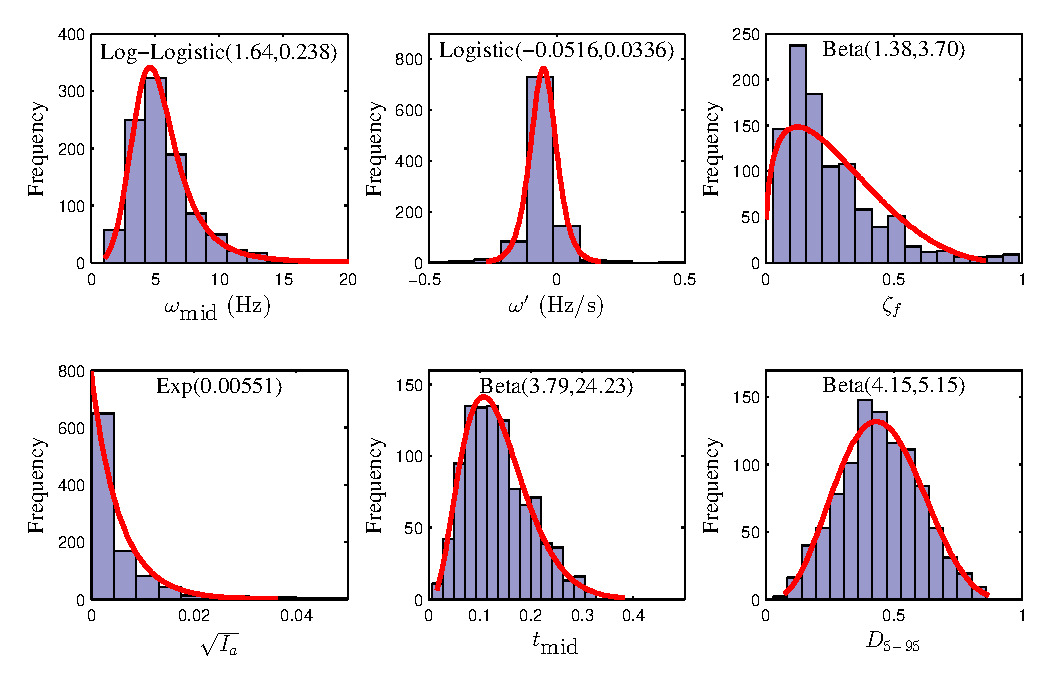
\includegraphics[width=12.5cm]{figs/histfit.eps}}
\caption{Histograms of the stochastic ground motion model parameters along with the fitted probability density function.}\label{fig:histfit}
\end{figure*}
% ================================================


% ================================================
\subsubsection{PC basis}
% ================================================
PC functional subspace selection may be formulated as a discrete variable selection problem that may be tackled through a Genetic Algorithm (GA) that minimizes the the Bayesian Information Criterion (``fitness'' function) (BIC; \citeNP{Ljung1999}):
%%
\beq \text{BIC} = -\ln (\hat{\sigma}_{\bld E}^2) + \frac{\ln (KT)}{K T} \cdot \dim{\bth}  \eeq
%%
where $\hat{\sigma}_{\bld E}^2$ designates the estimation of the residual sequence ${\bld E}$ variance, and $\dim{\bth}$ the number of independently adjusted  model parameters, that is the number of the deterministic coefficients of projection. Finally, $K T$ is the total number of data samples used for the estimation of the PC-NARX model. 

In order to illustrate this procedure consider an initial PC basis with total maximum degree $P = 2$ and $M = 3$ input random variables. The dimensionality of this basis will be equal to \cite{Blatman-Sudret2010}:
%%
$$ p = \frac{(M+P) !}{M! P !} = \frac{5!}{3!2!} = 10$$
%%
In order to represent all the functional subspaces included in this initial search space through a compact 10-bit binary vector, each multi-index vector ${\bld d}(j) \ (j =1,\ldots,10)$ may be represented by a single bit indicating the existence (1) or not (0) of the corresponding PC basis function in the specific model structure.


% ========================================================================
\section{PARAMETRIC REPRESENTATION OF SYNTHETIC EARTHQUAKES}
% ========================================================================

In the present study, the stochastic ground motion model proposed in \citeNP{Rezaeian-Kiureghian2010} is employed for the parametric representation of synthetic earthquake ground motion acceleration signals. According to this model the ground motion is produced by time-modulating a normalized filtered white noise process. In order to simulate the time-varying characteristics of both the temporal and spectral content of a real earthquake, the modulating function and the Impulse Response Filter (IRF) of the aforementioned model have non-stationary properties. 

More specifically, the non-stationary modulating function is defined as a gamma function of the following form: 
%%
\beq
q(t,{\bld \alpha}) = \alpha_1 t^{\alpha_2-1}\exp(-\alpha_3 t) 
\eeq
%%
where ${\bld \alpha}=[ \alpha_1, \alpha_2, \alpha_3 ]^{\mathsf T}$, with $\alpha_1 > 0$ the parameter of the process intensity, $\alpha_2> 1$ the parameter controlling the shape of the modulating function, and $\alpha_3 > 0$ the duration of the motion. The parameters of the modulating function, may be directly estimated from three time-domain characteristics of a ground motion accelerogram: \emph{i)} the expected Arias intensity $I_a$, that is a measure of the total energy contained in the motion, \emph{ii)} the effective duration of the motion $D_{5-95}$ (the time interval between the instants at which the 5 and 95\% of the expected Arias intensities are reached), and finally \emph{iii)} the time $t_{\text{mid}}$ at which 45\% level of the expected Arias intensity is reached.

On the other hand, the non-stationary IRF is given by the following expression:
%%
\beq
h[t-\tau] = \tfrac{\omega_f(\tau) e^{-\zeta_f \omega_f(\tau) (t-\tau)} \cdot \sin\bigl[ \omega_f(\tau)  (t-\tau) \sqrt{1-\zeta_f^2} \bigr] }{\sqrt{1-\zeta^2_f}} 
\eeq
%%
for $ \tau\leq t $, with $\zeta_f$ designating the damping ratio of the filter and $\omega_f(\tau)$ the filter's frequency. The latter is defined as $\omega_f(\tau) = \omega_{\text{mid}} + \omega'(\tau-t_{\text{mid}})$ with $\omega_{\text{mid}}$ representing the filter frequency at $t_{\text{mid}}$, and $\omega'$ the rate of change of the filter frequency with time. 

Therefore, given a target accelerogram, the parameters $\omega_{\text{mid}}, \omega', \zeta_f, I_a, D_{5-95}$, and $t_{\text{mid}}$ may be identified by matching the properties of the recorded motion with the corresponding statistical measures of the stochastic ground motion model \cite{Rezaeian-Kiureghian2010}. The identified model may be subsequently used for the generation of synthetic ground motion accelerograms with similar time-frequency characteristics with that of the real recorded motion. 


In a similar way, a pdf may be identified for each of the stochastic ground motion model parameters in order to represent not a single but a set of real earthquake accelerograms. This procedure is presently applied for the modeling of the 3551 ground motion signals of the PEER database (horizontal components only; \citeNP{Peer2012}). From the identified sets of parameters, only the 1000 with the best model fitting are kept for the subsequent analysis. The resulting histograms for the identified parameters and the fitted pdfs are shown in figure \ref{fig:histfit} ($D_{5-95}$ and $t_{\text{mid}}$ are shown in normalized discrete time $t/T$). 


% ================================================
\section{NUMERICAL EXAMPLE}
% ================================================

A FE model of a building frame structure is presently considered for the validation of the introduced method (figure \ref{fig:ShearFrame}). The identification of the frame's metamodel is based on recordings of the horizontal acceleration of the top floor of the building measured at node 12 ($y[t] =\alpha_{12}[t] $; figure \ref{fig:ShearFrame}) obtained by the time history loading of the FE model with various synthetic earthquake ground motion signals. 

% Figure
% ================================================
\begin{figure}[t!]
\centering
\includegraphics[height = 270pt]{figs/ShearFrame5storey.eps}
\caption{The five-storey shear frame model.}\label{fig:ShearFrame}
\end{figure}
% ================================================

% Table
% ================================================
\begin{table} 
\caption{Geometric and mechanical properties of the five-storey shear frame model.}\label{tab:con_prop}
\tabletext{
\begin{tabular}{llll}\hline
\multicolumn{2}{l}{Geometric}& \multicolumn{2}{l}{Mechanical}\\[-6pt]
\multicolumn{2}{l}{\hrulefill}& & \\
Cross-sectional area & \hspace{-0.2cm} cm$^2$ & & \\\hline
1$^{\text{st}}$ storey columns & \hspace{-0.2cm} 900 & Poisson ratio & \hspace{-0.2cm} 0.29 \\
2$^{\text{nd}}$ storey columns & \hspace{-0.2cm} 625 & Density (kg/m$^3$)  & \hspace{-0.2cm} 7850\\
3$^{\text{rd}}$ storey columns & \hspace{-0.2cm} 400 & Yield stress (MPa) & \hspace{-0.2cm} 200\\
4$^{\text{th}}$ storey columns & \hspace{-0.2cm} 225 & Tangent modulus (GPa) & \hspace{-0.2cm} 10 \\
5$^{\text{th}}$ storey columns & \hspace{-0.2cm} 100 & & \\ 
Horizontal beams & \hspace{-0.2cm} 100 & & \\\hline
\end{tabular}}
\end{table}
% ================================================

The elements of the shear frame are considered to have square cross section and being made of steel with isotropic behavior described by a bilinear stress-strain curve. The constant, characterized by negligible uncertainty, mechanical and geometric properties of the structure are summarized in table \ref{tab:con_prop}. On the other hand, the steel's Young modulus $E$ is considered to be uncertain, modeled by a random variable following a uniform distribution $ E \sim {\mathcal U}(180,220)$ (GPa). 

The uncertain input parameter vector of this numerical example, includes also the stochastic ground motion model parameters $\omega_{\text{mid}}, \omega', I_a$, and $D_{5-95}$ which follow the distributions indicated in figure \ref{fig:histfit}. For this case study the IRF filter damping ratio $\zeta_f$ is considered constant and equal to $0.1$ for all synthetic earthquake accelerograms. Moreover, the high correlation between the $D_{5-95}$ and $t_{\text{mid}}$ variables admits the usage of a linear relationship between this two variables (see figure \ref{fig:D545_D595}). Thus, using a least square fitting $t_{\text{mid}}$ is considered always equal to $0.3075 D_{5-95}$.



% Figure
% ================================================
\begin{figure}
\centering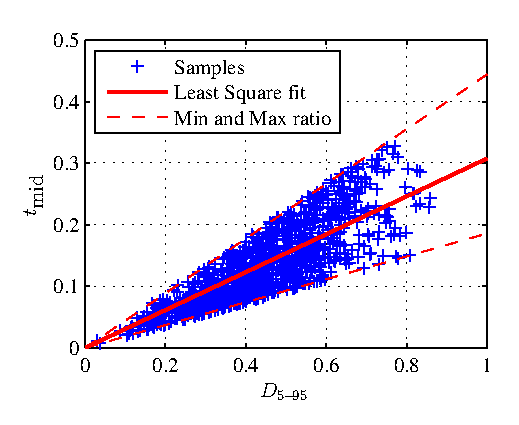
\includegraphics[width=6.75cm]{figs/D545_D595.eps}
\caption{Identified values of $D_{5-95}$ versus $t_{\text{mid}}$ for the accelerograms of the PEER ground motion database.}\label{fig:D545_D595}
\end{figure}
% ================================================


Summarizing, in total five independent input random variables with known pdfs are considered for this metamodeling problem (see table \ref{tab:input_vars}). 

% Table
% ================================================
\begin{table}
\caption{Random input variables.}\label{tab:input_vars}
\tabletext{
\begin{tabular}{lll} \hline 
Variable 				& Distribution 	& pdf parameters \\ [1pt] \hline
E (GPa)  				& Uniform 		& $\min = 180$, $\max = 220$ \\
$\omega_{\text{mid}}$ (Hz) & Log-Logistic 	& $\alpha = 1.64 $, $\beta = 0.238 $ \\
$\omega'$ (Hz/s)		& Logistic 		& $\mu = -0.0516 $, $\sigma = 0.0336 $\\ 
$\sqrt{I_a}$ 					& Exponential 	& $\mu = 0.00551 $\\
$D_{5-95}$ & Beta & $\alpha = 4.15, \beta = 5.15$\\ \hline
\end{tabular}}
\end{table}
% ================================================



% ================================================
\subsection{Simulation experiments}
% ================================================

A total number of 200 simulations is conducted ($K =200$) for a corresponding number of input random vector realizations $\bxi_k (k=1,2,\ldots,200)$ sampled by the LHS method. The values of the sampled variables along with their histograms are shown in figure \ref{fig:sim_inputs}.

% Figure
% ================================================
\begin{figure}
\centering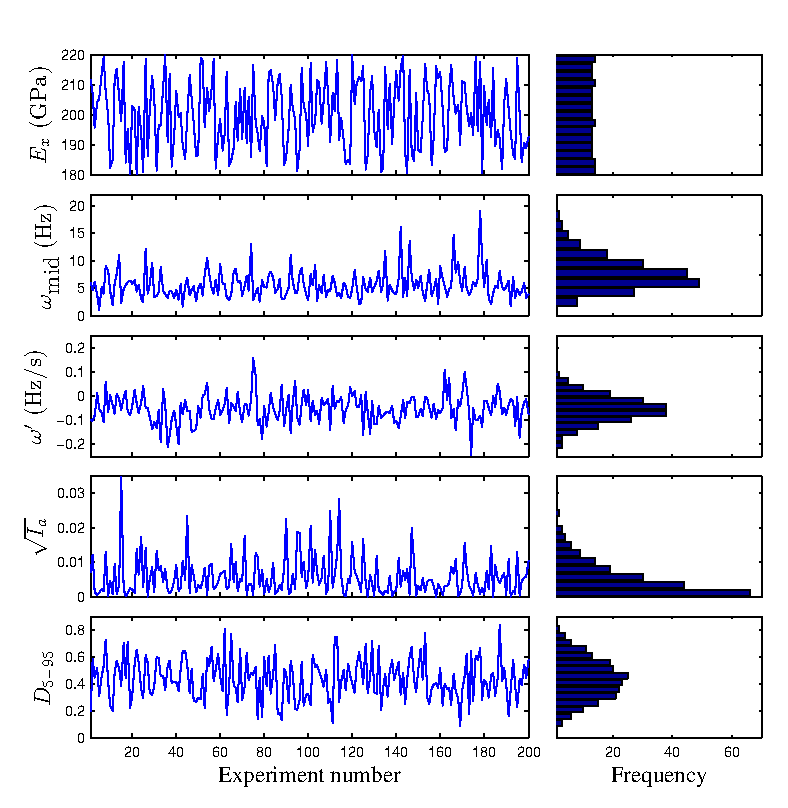
\includegraphics[width=9cm]{figs/input_pars.eps}
\caption{The input random vector realizations for the 200 simulations conducted.}\label{fig:sim_inputs}
\end{figure}
% ================================================


For each simulation experiment, the shear frame model is excited by a synthetic ground motion accelerogram applied in the x-axis direction (sampling frequency $f_s = 40$ Hz; 1000 number of samples for each accelerogram). The Peak Ground Acceleration (PGA) values of the synthetic accelerograms varies between 0.16 and 0.67 g with all the levels of this range being capable of exciting the nonlinear dynamics of the FE model (for instance see figure \ref{fig:simulations}(d)). The acceleration of the FE model measured at node 12, along with the corresponding shear stress and top floor displacement recordings for the first three simulations are also shown in figure \ref{fig:simulations}.


\subsection{PC-NARX metamodel identification}

For the metamodel structure selection problem PC-NARX models with $n_a = n_b = 10 $ are considered, while the appropriate nonlinear terms $g_i({\bld z}[t])$ are searched among polynomial functions of the following form:
%
$$ g_i({\bld z}[t]) = z_{j_1}^{\ell_1}[t] \cdot z_{j_2}^{\ell_2}[t]$$
%
with $\ell_1,\ell_2 = 0,\ldots 3$, $\ell_1 + \ell_2 \leq 3$, and ${\bld z}[t] = \left[ \ y[t-1], \ldots, y[t-10], x[t], x[t-1], \ldots, x[t-10]\ \right]^{\mathsf{T}}$. The application of the OFR algorithm for the selection of the most significant terms leads to the selection of the following 46 linear and nonlinear terms:
%
$y[t-1], \ldots,y[t-10], x[t], x[t-1], \ldots,x[t-10],$ \vspace{0.2cm} \\
%
$y[t-1]\cdot y^2[t-2], \ldots, y[t-1]\cdot y^2[t-10],$ \vspace{0.2cm} \\
%
$y^2[t-1]\cdot y[t-2], \ldots, y^2[t-1]\cdot y[t-10],$ \vspace{0.2cm} \\
$y^3[t-1], y^3[t-2], y^3[t-3].$

The GA optimization procedure outlined in section 2.2.2 is then utilized for the selection of the appropriate PC basis functions. The initial search space is defined by the truncated set of multivariate Legendre polynomials basis functions of maximum total degree equal to three -- it is noted that the input random variables listed in table \ref{tab:input_vars} are first transformed into standard uniform variables by using the inverse cumulative density functions of the corresponding pdfs. The minimization of the BIC criterion through the GA leads to the selection of nine basis functions. 


% Figure
% ================================================
\begin{figure}[t!]
\centerline{
\begin{picture}(255,280)
\put(-2,0){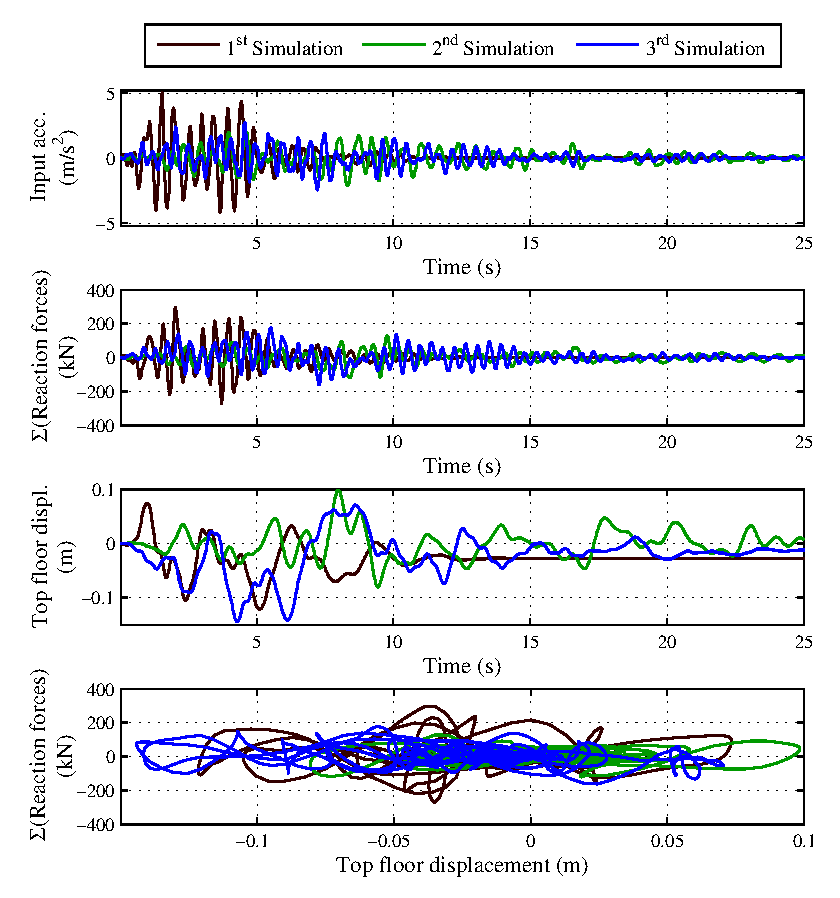
\includegraphics[width=260pt]{figs/SF2D_simulations.eps}}
\put(232,244){(a)}
\put(232,180){(b)}
\put(232,115){(c)}
\put(232,50){(d)}
\end{picture}}
\caption{Input-output data from the first three simulation experiments: (a) Input excitation signals $x_1^T, x_2^T$ and $x_3^T$, (b) node 12 acceleration response signals $y_1^T, y_2^T$ and $y_3^T$, (c) top floor displacement measured at node 12, and (d) the shear stresses versus top floor displacements.} \label{fig:simulations}
\end{figure}
% ================================================

The multi-indices vectors of these functions are given in table \ref{tab:PCindx}. It should be observed that according to these results the PC-NARX metamodel parameters $\theta_i$ and thus the dynamic properties of the corresponding numerical model seem to be highly sensitive to the input variable $\omega_{\text{mid}}$ which defines the dominant frequency of the synthetic ground motion signal used for the excitation of the FE model. The significant sensitivity to the Young modulus variables comes also as no surprise since it is directly related to the dynamics of the modeled structure. On the other hand, the results of table \ref{tab:PCindx} indicate no sensitivity of the metamodel parameters $\theta_i$ on the rate of change of the synthetic ground motion frequency $\omega'$. Finally, interesting is the result that the PC basis functions indicate low sensitivity to the input variable $\sqrt{I_a}$ which controls the intensity of the ground motion. However, this fact may attributed to the relatively narrow PGA range of the synthetic earthquakes. 

The estimated, based on the PE method, PC-NARX metamodel is also successfully validated with respect to the assumptions on the residual sequences (see equation \ref{eq:assumptions}) through the auto-correlation and cross-correlation functions. The uncrosscorrelatedness between the residual sequences $e_k^T (k=1,\ldots,K)$ may be illustrated through the almost diagonal covariance matrix $\mbox{cov}(\hat{\bld e}_{k_1}, \hat{\bld e}_{k_2})$ depicted in figure \ref{fig:covariance}.   

%%
\begin{table}[t!]
\caption{Multi-indices vectors of the selected PC basis functions.}\label{tab:PCindx}
\tabletext{
\begin{tabular}{cccccc}\hline
& $\xi_1 (E)$ & $\xi_2 (\omega_{\text{mid}})$ & $\xi_3 (\omega')$ & $\xi_4 (I_a)$ & $\xi_5 (D_{5-95})$\\ \hline
${\bld d}{(1)}$ & 0 & 0 & 0 & 0 & 0 \\ 
${\bld d}{(2)}$ & 1 & 0 & 0 & 0 & 0 \\
${\bld d}{(3)}$ & 0 & 1 & 0 & 0 & 0 \\  
${\bld d}{(4)}$ & 0 & 0 & 0 & 0 & 1 \\ 
${\bld d}{(5)}$ & 1 & 0 & 0 & 1 & 0 \\ 
${\bld d}{(6)}$ & 0 & 1 & 0 & 0 & 1 \\ 
${\bld d}{(7)}$ & 0 & 2 & 0 & 0 & 0 \\ 
${\bld d}{(8)}$ & 1 & 2 & 0 & 0 & 0 \\ 
${\bld d}{(9)}$ & 0 & 3 & 0 & 0 & 0 \\ \hline
\end{tabular}}\vspace{-0.1cm}
\end{table}



% Figure
% ================================================
\begin{figure}
\centering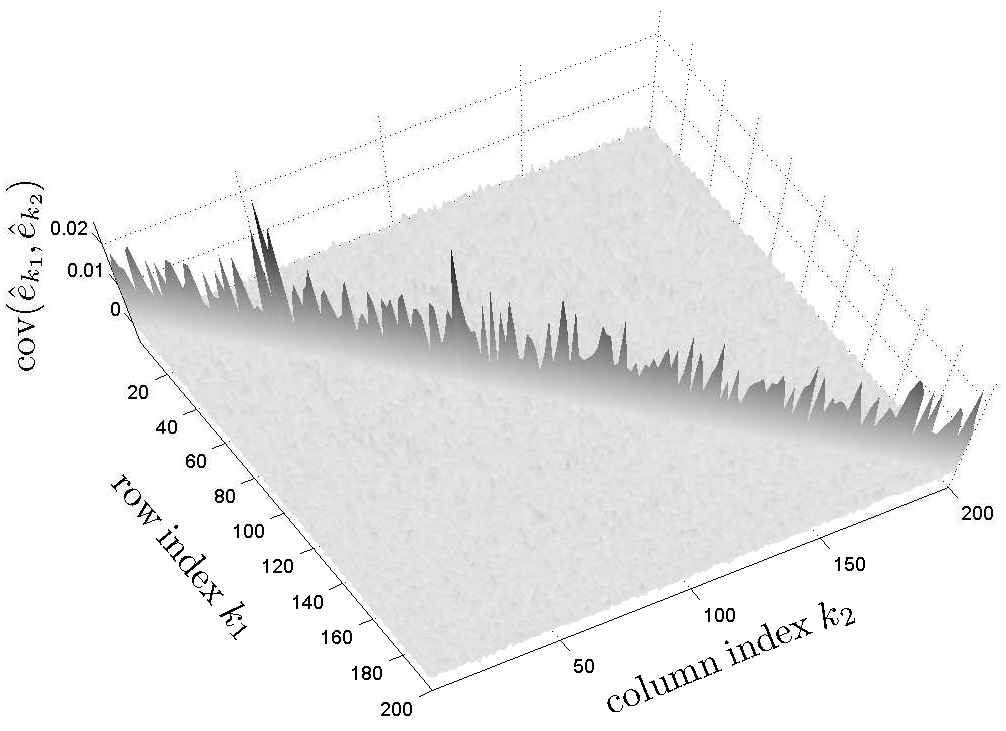
\includegraphics[width=7cm]{figs/covariance.eps}
\caption{Covariance matrix between the estimated PC-NARX model residual sequencies $\hat{\bld e}_k (k=1,\ldots,K)$.}\label{fig:covariance}
\end{figure}
% ================================================

The performance of the estimated metamodel is assessed through its application for both prediction and simulation of the dynamic response of the FE model excited by the N-S component of the El Centro earthquake accelerogram. The Young modulus of the shear frame for this test case is selected as $E = 200$ GPa, while the rest of the input random variables are estimated from the actual accelerogram as $\omega_{\text{mid}} = 3.8227$ (Hz), $\omega'=  -0.0202$ (Hz/s), $\sqrt{I_a} = 0.0188$ and $D_{5-95} = 0.4544$ (sampling frequency equal to 40 Hz; 2688 samples). 

The predictions of the PE-based and the simulations of the SE-based estimated PC-NARX metamodels are contrasted to the dynamic response of the numerical model in figure \ref{fig:preds} (first 600 samples; for the SE method: Levenberg-Marquardt algorithm, {\em lsqnonlin} MATLAB function, TolFun = $1\times 10^{-6}$, TolX = $1\times 10^{-9}$). As it may be observed, the estimated metamodel is capable of reproducing the dynamic response of the numerical model with good accuracy. It is worth noting that these results are obtained for an excitation signal for which the assumptions of $\zeta_f = 0.1$, and $t_{\text{mid}} = 0.3075 D_{5-95}$ are no longer valid. Finally, it should be added that the PC-NARX based simulated response was calculated more than 100 times faster than that of the FE model.  

% ===============================================
\section{CONCLUSIONS}
% ===============================================
This work introduces a methodology for the metamodeling of large scale numerical models with uncertain parameters and under stochastic excitation. The metamodel utilized is based on Polynomial Chaos Nonlinear ARX models with parameters which are random variables depending on the input random variables, with this dependency being described by their expansion of a properly selected polynomial chaos basis.
 
The method is applied for the metamodling problem of a five-storey shear frame FE model subject to synthetic earthquake ground motion accelerograms. Input random variables are used to describe the uncertainties of both the material properties of the simulated structure and the input excitation signals. The estimation of the PC-NARX model is based on a set of 200 input-output simulation data sets with the results being very promising. 

% Figure
% ================================================
\begin{figure}[t!]
\centering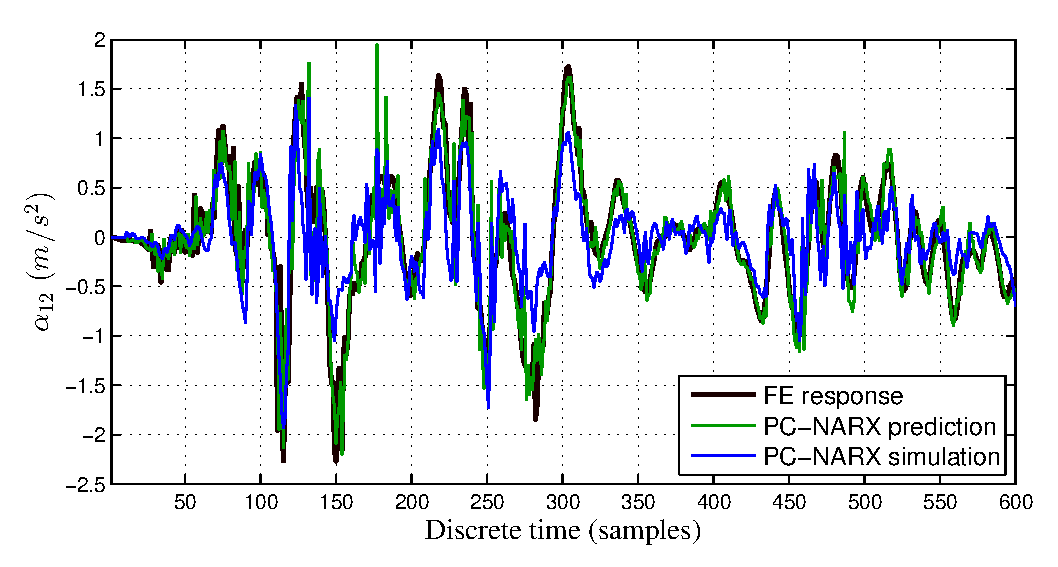
\includegraphics[width=9cm]{figs/preds_sims.eps}
\caption{The dynamic response of the shear frame FE model and the corresponding PC-NARX based one-step-ahead-predictions and simulation signals for the El Centro earthquake time history loading.}\label{fig:preds}
\end{figure}
% ================================================


\bibliographystyle{chicaco}
\bibliography{ICOSSAR2013database}

\end{document}
